\subsection{Mengirimkan pesan}
Halaman ini hanya dapat diakses oleh pengguna yang sudah terdaftar dan masuk/\textit{login} ke dalam sistem. Pada halaman ini terdapat elemen-elemen halaman \textit{chatting} pada umumnya, yaitu elemen \textit{input} pesan, tombol Kirim, dan riwayat beberapa pesan sebelumnya. Spesifikasi kasus penggunaan dapat dilihat pada tabel \ref{uc04.04}.\\
\indent Terdapat logika \textit{view} dan alur proses khusus dikarenakan sifat pengiriman dan penerimaan pesan yang realtime, sehingga dibangun diatas Node.js dan menggunakan Socket.io. Sebagai ringkasan dari ketiga logika tersebut, visualisasi pada gambar \ref{cdvis.04-04} akan membantu menggambarkan keseluruhan proses logika secara ringkas. Masing-masing logika tersebut dapat dijabarkan sebagai berikut:
	\begin{enumerate}
		\item Logika \textit{back-end} ditulis menggunakan PHP yang dicantumkan dalam kode sumber \ref{cdbe.04-04}; 
		\item Logika \textit{view} ditulis menggunakan jQuery yang dicantumkan dalam kode sumber \ref{cdjq.04-04}; dan
		\item Logika proses pengiriman \& penerimaan pesan, berjalan diatas socket yang berjalan diatas Node.js dengan bantuan Socket.io yang dicantumkan dalam kode sumber \ref{cdsoc.04-04}
	\end{enumerate}

\begin{figure}[H]
\centering
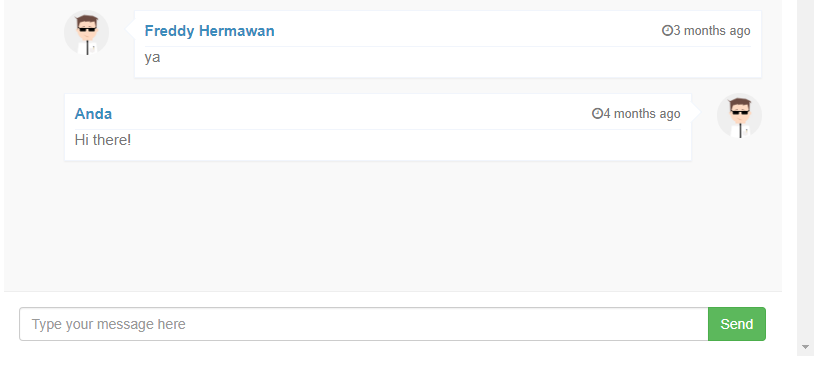
\includegraphics[width=\textwidth]{images/bab4/ui/04-04.png}
\caption{Halaman Antarmuka Implementasi Kasus Penggunaan Mengirimkan Pesan}
\label{ui.04-04}
\end{figure}

\begin{lstlisting}[label=cdbe.04-04,style=php,caption=Kode Sumber \textit{Back-end} Mengirimkan Pesan]
/*	file : app/Http/Controllers/ChatController */
public function chat($id_user)
	/*	method : GET */

    if(intval($id)){
        $data['from'] = Auth::user()->id;
        $data['to'] = $id;
        $data['user'] = User::findOrFail($id);

        if($data['user']){
            return view('pages.user.chat', $data);
        }
    }

    /* 	Jika ada parameter error, 
    	redirect kembali dengan pesan error */
    return redirect('/')->with('error','User yang anda cari tidak dapat ditemukan.');

}
\end{lstlisting}

\begin{lstlisting}[label=cdsoc.04-04,style=htmlcssjs,caption=Kode Sumber Logika View Lelang (menggunakan Node.js)]
/*	
	file : chatserver\_https.js 
	menggunakan dependencies : socketio (ioServer), jwt, https, http, fs dan express
*/
socket.on('join-room', function(room) {
	/*
		fungsi ini dipanggil saat
		pertama kali pengguna membuka halaman chat
		dimana pengguna masuk ke dalam room percakapan
	*/
    var parsedRoom = parseRoom(room);


	/*
		Jika room ini belum pernah dimasuki/ chat perdana
		maka ditambahkan ke tabel joinedroom
	*/
    insertToRoomCollection(roomcollection, parsedRoom, false, function() {
        socket.join(parsedRoom.room);

        // 
        var cb = function(err, chat) {
          if (chat!=[]){
            socket.emit('chathistory', chat);
          }
        };

		/*
			Broadcast 5 percakapan terakhir
			dalam room tersebut
			ke pengguna yang baru saja join room.
		*/
        collection.find({ room : parsedRoom.room }).sort({ sent : -1 }).limit(50).toArray(cb);
    });

});


socket.on('send', function(data) {
	/*
		parameter yang masuk adalah JSON dengan konstruksi berikut :
		{ room: , body : }
	*/

    var msgParse = JSON.parse(data);
    var parsedRoom = parseRoom(msgParse.room);

    //constructing inserting query
    var insertQuery = {
        room : parsedRoom.room,
        sender : parsedRoom.from,
        msg : msgParse.body,
        sent : new Date()
    };

    //insert kedalam database
    collection.insert(insertQuery, function(err, o) {
        var ll = parsedRoom.from.toString();
        if (err) io.to(ll).emit('send-status', { status : false});
        else io.to(ll).emit('send-status', { status : true });
    });

    // update room information
    // bahwa room ini sudah diperbarui
    insertToRoomCollection(roomcollection, parsedRoom, true);

    //broadcast ke user yang tergabung ke room percakapan
    io.to(parsedRoom.room).emit('new-msg', insertQuery);

});

\end{lstlisting}

\begin{lstlisting}[label=cdjq.04-04,style=htmlcssjs,caption=Kode Sumber Logika Pengiriman \& Penerimaan Pesan (menggunakan jQuery)]
var room = '{{ Auth::user()->id }}-{{ $user->id }}';
var prepstat = '{ "room" : "' + room + '", "body" : "';
var closetag ='"}';

/* 
	Masuk ke dalam room
 */
socket.emit('join-room', room);


/* 
	Menerima riwayat perpesanan dan merender pesan-pesan tersebut ke view dengan fungsi bantu appendNewChat()
 */
socket.on('chathistory', function(data){
    console.log(data);
    $(data).each(function(index,value){
        appendNewChat(value);
    });
});

$('.sendMessage').click(function(){
	/*	
		constructing JSON message 
		concate previous statement with message's body
		and close tag
		*/
    var msg = prepstat + $('.body').val() + closetag ;

    /* disable input pesan untuk sementara */
    $(".body").attr("disabled", true);

    /*kirimkan pesan */
    socket.emit('send', msg );

    /* menunggu status pengiriman pesan */
    socket.on('send-status', function(data){
    	/* Jika gagal, enable input pesan dengan tidak menghapus pesan yang belum jadi dikirimkan sebelumnya */
        if(!data.status){
            swal('Oops','Pesan anda tidak dapat terkirim, silahkan coba lagi','error');
        }
        /* Jika sukses, enable input pesan dengan elemen input pesan yang sudah dikosongkan */
        else if(data.status){
            $('.body').val('');
        }

    }, function(){
        $(".body").attr("disabled", false);
    });
});

/* 
	Bagian ini dieksekusi saat ada pesan baru masuk ke dalam room. appendNewChat() adalah fungsi bantu merender view untuk menampilkan pesan baru
 */
socket.on('new-msg', function (value) {
    appendNewChat(value);
});
\end{lstlisting}